\chapter{Формы}

Мы уже упоминали граничное условие: когда данные приходят в приложение или покидают его,
мы должны их проверить. Вероятно, наиболее сложная проверка происходит в формах.
Программировать формы --- сложно; в идеальном мире мы хотели бы уметь:

\begin{itemize}
\item убеждаться, что данные валидны; % FIXME: valid --- действительны, годны, зачетны :)
\item преобразовать строковые данные формы в типы данных Haskell; % FIXME: marshal --- ?
\item генерировать код HTML для отображения формы;
\item генерировать Javascript, выполняющий валидацию на стороне клиента и предоставляющий
более дружелюбные виджеты, такие как,например, выбор даты;
\item строить более сложные формы, объединяя вместе более простые;
\item автоматически присваивать полям имена, для которых гарантируется уникальность.
\end{itemize}

Пакет \lstinline'yesod-form' предоставляет все эти возможности с простым декларативным
API. Он строится на виджетах Yesod, чтобы упростить дизайн форм и надлежащее применение
Javascript. И, как и остальной Yesod, использует систему типов Haskell для обеспечения
корректной работы.
% FIXME: styling (of forms) --- дизайн (форм)
% FIXME: род слова Yesod -- мужской? 

\section{Краткий обзор}

% FIXME: род i18n --- женский (интернационализация?)
% FIXME: parsed --- ???
\begin{lstlisting}
{-# LANGUAGE QuasiQuotes, TemplateHaskell, MultiParamTypeClasses,
    OverloadedStrings, TypeFamilies #-}
import Yesod
import Yesod.Form.Jquery
import Data.Time (Day)
import Data.Text (Text)
import Control.Applicative ((<$>), (<*>))

data Synopsis = Synopsis

mkYesod "Synopsis" [parseRoutes|
/ RootR GET
/person PersonR POST
|]

instance Yesod Synopsis

-- Указывает приложению использовать стандартные английские сообщения
-- Если вам нужна i18n, вы можете предоставить функцию перевода
instance RenderMessage Synopsis FormMessage where
    renderMessage _ _ = defaultFormMessage

-- И указывает, где найти библиотеки jQuery. Мы будем использовать значение
-- по умолчанию, указывающее на Google CDN
instance YesodJquery Synopsis

-- Тип данных, который мы хотим получить из формы
data Person = Person
    { personName :: Text
    , personBirthday :: Day
    , personFavoriteColor :: Maybe Text
    , personEmail :: Text
    , personWebsite :: Maybe Text
    }
  deriving Show

-- Объявление формы. Сигнатура типа несколько пугающая, но вот её обзор:
--
-- * Параметр Html используется для кодирования некоторой дополнительной
-- информации. См. обсуждение runFormGet и runFormPost ниже для 
-- дополнительного объяснения
--
-- * Как обычно, у нас есть типы под- и главного сайта
--
-- * FormResult может находиться в трех состояниях: FormMissing (нет
-- доступных данных), FormFailure (некорректные данные) и FormSuccess
--
-- * Widget "--- отображаемая форма для вставки на страницу
--
-- Обратите внимание, что шаблон сайта предоставляет удобный синоним типа
-- Form, так что наша сигнатура может быть переписана как:
-- > personForm :: Form Person
--
-- Для наших целей лучше видеть полную версию
personForm :: Html -> MForm Synopsis Synopsis (FormResult Person, Widget)
personForm = renderDivs $ Person
    <$> areq textField "Name" Nothing
    <*> areq (jqueryDayField def
        { jdsChangeYear = True -- give a year dropdown
        , jdsYearRange = "1900:-5" -- 1900 till five years ago
        }) "Birthday" Nothing
    <*> aopt textField "Favorite color" Nothing
    <*> areq emailField "Email address" Nothing
    <*> aopt urlField "Website" Nothing

-- Обработчик GET-запроса отображает форму
getRootR :: Handler RepHtml
getRootR = do
    -- Generate the form to be displayed
    (widget, enctype) <- generateFormPost personForm
    defaultLayout [whamlet|
<p>The widget generated contains only the contents of the form, not the form tag itself.
So...
<form method=post action=@{PersonR} enctype=#{enctype}>
    ^{widget}
    <p>It also doesn't include the submit button.
    <input type=submit>
|]

-- Обработчик POST-запроса обрабатывает форму. Если обработка успешно 
-- завершилась, он отображает данные переданного человека. Иначе -- снова
-- форму с сообщениями об ошибке.
postPersonR :: Handler RepHtml
postPersonR = do
    ((result, widget), enctype) <- runFormPost personForm
    case result of
        FormSuccess person -> defaultLayout [whamlet|<p>#{show person}|]
        _ -> defaultLayout [whamlet|
<p>Invalid input, let's try again.
<form method=post action=@{PersonR} enctype=#{enctype}>
    ^{widget}
    <input type=submit>
|]

main :: IO ()
main = warpDebug 3000 Synopsis
\end{lstlisting}

\section{Виды форм}

Перед тем, как рассмотреть сами типы, начнем с обзора разных видов форм. Имеются три типа
форм:

\subsection{Аппликативные}
Наиболее широко используемые (они были использованы выше в примере). Аппликативные формы
позволяют нам объединять сообщения об ошибках друг с другом, сохраняя при этом
декларативный высокоуровневый подход. Более детальную информацию об аппликативном подходе
можно почерпнуть в Haskell-вики.

\subsection{Монадические}
Более мощная альтернатива аппликативным. Гибкость достигается за счет несколько большей
многословности. Бывают полезны, если необходимо создать форму, которая не укладывается в
стандартный двухстолбцовый формат.

\subsection{Для ввода}
Используются только для ввода данных. Не генерируют никакого HTML для получения ввода
пользователя. Полезны для взаимодействия с уже существующими формами.

К тому же, существует некоторое число переменных для каждого вида форма, а также поля,
которые вам, возможно, захочется установить:
\begin{itemize}
\item Это поле обязательное или опциональное?
\item Данные должны передаваться методом GET или POST?
\item У него есть значение по-умолчанию или нет?
\end{itemize}

Основная цель заключается в том, чтобы минимизировать число определений полей и позволить
им быть полезными в как можно большем числе контекстов. В следствии этого мы добавляем
несколько слов для каждого поля. В обзоре, вы наверное заметили такие штуки как
\lstinline'areq' и лишний параметр \lstinline'Nothing'. Мы обсудим зачем они нужны в
рамках данной главы, а сейчас пока можете считать, что сделав эти поля явными, мы можем
переиспользовать одиночные поля (как, например, \lstinline'intField') несколькими
различными способами.

Замечание по поводу именования. Каждая форма имеет однобуквенный префикс (A, M или I)
который используется в нескольких местах, как например в \lstinline'MForm'. Мы также
будем использовать \lstinline'req' и \lstinline'opt' для обозначения обязательности и
опциональности соответственно. Так мы можем создавать обязательное аппликативное поле с
помощью \lstinline'areq' или оциональное поле для вода данных и помощью \lstinline'iopt'.

\section{Типы}

Модуль \lstinline'Yesod.Form.Types' определяет несколько типов.Давайте начнем с самыз
простых:

\subsection{Enctype}

The encoding type, either UrlEncoded or Multipart. This datatype declares an instance of
ToHtml, so you can use the enctype directly in Hamlet.

\subsection{Env}

Maps a parameter name to a list of values.

\subsection{FileEnv}

Maps a parameter name to the associated uploaded file.

\subsection{Ints}

As mentioned in the introduction, yesod-form automatically assigns a unique name to each
field. Ints is used to keep track of the next number to assign.

\subsection{FormResult}

Has one of three possible states: FormMissing if no data was submitted, FormFailure if
there was an error parsing the form (e.g., missing a required field, invalid content), or
FormSuccess if everything went smoothly.

Next we have three datatypes used for defining individual fields.

A field is a single piece of information, such as a number, a string or an email address.
Fields are combined together to build forms.

\subsection{Field}

Defines two pieces of functionality: how to parse the text input from a user into a
Haskell value, and how to create the widget to be displayed to the user. yesod-form
defines a number of individual Fields in Yesod.Form.Fields.

\subsection{FieldSettings}

Basic information on how a field should be displayed, such as the display name, an
optional tooltip, and possibly hardcoded id and name attributes. (If none are provided,
they are automatically generated.)

FieldSettings provides an IsString instance, so when you need to provide a FieldSettings
value, you can actually type in a literal string. That's how we interacted with it in the
synopsis.

\subsection{FieldView}

An intermediate format containing a bunch of view information on a field. This is hardly
ever used directly by the user, we'll see more details later.

And finally, we get to the important stuff: the forms themselves. There are three types
for this: MForm is for monadic forms, AForm for applicative and IForm (declared in IForm)
for input. MForm is actually a type synonym for a monad stack that provides the following
features:
\begin{itemize}
\item A Reader monad giving us the parameters (Env and FileEnv), the master site
argument and the list of languages the user supports. The last two are used for i18n (more
on this later).
\item A Writer monad keeping track of the Enctype. A form will always be UrlEncoded,
unless there is a file input field, which will force us to use multipart instead.
\item A State monad holding an Ints to keep track of the next unique name to produce.
\end{itemize}
An AForm is pretty similar. However, there are a few major differences:
\begin{itemize}
\item It produces a list of FieldViews. This allows us to keep an abstract idea of the
form display, and then at the end of the day choose an appropriate function for laying it
out on the page. In the synopsis, we used renderDivs, which creates a bunch of div tags.
Another option would be renderTable.

\item It does not provide a Monad instance. The goal of Applicative is to allow the entire
form to run, grab as much information on each field as possible, and then create the final
result. This cannot work in the context of Monad.
\end{itemize}
An IForm is even simpler: it returns either a list of error messages or a result.

\section{Converting}

"But wait a minute," you say. "You said the synopsis uses applicative forms, but I'm sure
the type signature said MForm. Shouldn't it be Monadic?" That's true, the final form we
produced was monadic. But what really happened is that we converted an applicative form to
a monadic one.

Again, our goal is to reuse code as much as possible, and minimize the number of functions
in the API. And Monadic forms are more powerful than Applicative, if more clumsy, so
anything that can be expressed in an Applicative form could also be expressed in a Monadic
form. There are two core functions that help out with this: aformToForm converts any
applicative form to a monadic one, and formToAForm converts certain kinds of monadic forms
to applicative forms.

"But wait another minute," you insist. "I didn't see any aformToForm!" Also true. The
renderDivs function takes care of that for us.

\subsection{Create AForms}

Now that I've (hopefully) convinced you that in our synopsis we were really dealing with
applicative forms, let's have a look and try to understand how these things get created.
Let's take a simple example:

\begin{lstlisting}
data Car = Car
    { carModel :: Text
    , carYear :: Int
    }
  deriving Show

carAForm :: AForm Synopsis Synopsis Car
carAForm = Car
    <$> areq textField "Model" Nothing
    <*> areq intField "Year" Nothing

carForm :: Html -> MForm Synopsis Synopsis (FormResult Car, Widget)
carForm = renderTable carAForm

getCarR :: Handler RepHtml
getCarR = do
    ((result, widget), enctype) <- runFormGet carForm
    case result of
        FormSuccess car -> defaultLayout [whamlet|<p>#{show car}|]
        _ -> defaultLayout [whamlet|
<form method=get action=@{CarR} enctype=#{enctype}>
    <table>
        ^{widget}
    <input type=submit>
|]
\end{lstlisting}

Here, we've explicitly split up applicative and monadic forms. In carAForm, we use the
<\$> and <*> operators. This should not be surprising; these are almost always used in
applicative-style code. And we have one line for each record in our Car datatype. Perhaps
unsurprisingly, we have a textField for the Text record, and an intField for the Int
record.

Let's look a bit more closely at the areq function. Its (simplified) type signature is
Field a -> FieldSettings -> Maybe a -> AForm a. So that first argument is going to
determine the datatype of this field, how to parse it, and how to render it. The next
argument, FieldSettings, tells us the label, tooltip, name and ID of the field. In this
case, we're using the previously-mentioned IsString instance of FieldSettings.

And what's up with that Maybe a? It provides the optional default value. For example, if
we want our form to fill in "2007" as the default car year, we would use areq intField
"Year" (Just 2007). We can even take this to the next level, and have a form that takes an
optional parameter giving the default values.

\subsection{Form with default values}

\begin{lstlisting}
carAForm :: Maybe Car -> AForm Synopsis Synopsis Car
carAForm mcar = Car
    <$> areq textField "Model" (carModel <$> mcar)
    <*> areq intField "Year" (carYear <$> mcar)

carForm :: Html -> MForm Synopsis Synopsis (FormResult Car, Widget)
carForm = renderTable (carAForm $ Just $ Car "Forte" 2010)

getCarR :: Handler RepHtml
getCarR = do
    ((result, widget), enctype) <- runFormGet carForm
    case result of
        FormSuccess car -> defaultLayout [whamlet|<p>#{show car}|]
        _ -> defaultLayout [whamlet|
<form method=get action=@{CarR} enctype=#{enctype}>
    <table>
        ^{widget}
    <input type=submit>
|]
\end{lstlisting}

\section{Optional fields}

Suppose we wanted to have an optional field (like the car color). All we do instead is use
the aopt function.

\subsection{Optional fields}

\begin{lstlisting}
data Car = Car
    { carModel :: Text
    , carYear :: Int
    , carColor :: Maybe Text
    }
  deriving Show

carAForm :: AForm Synopsis Synopsis Car
carAForm = Car
    <$> areq textField "Model" Nothing
    <*> areq intField "Year" Nothing
    <*> aopt textField "Color" Nothing

carForm :: Html -> MForm Synopsis Synopsis (FormResult Car, Widget)
carForm = renderTable carAForm

getCarR :: Handler RepHtml
getCarR = do
    ((result, widget), enctype) <- runFormGet carForm
    case result of
        FormSuccess car -> defaultLayout [whamlet|<p>#{show car}|]
        _ -> defaultLayout [whamlet|
<form method=get action=@{CarR} enctype=#{enctype}>
    <table>
        ^{widget}
    <input type=submit>
|]
\end{lstlisting}

And like required fields, the last argument is the optional default value. However, this
has two layers of Maybe wrapping. This may seem redundant (and it is), but it makes it
much easier to write code that takes an optional default form parameter, such as in the
next example.

\subsection{Default optional fields}

\begin{lstlisting}
data Car = Car
    { carModel :: Text
    , carYear :: Int
    , carColor :: Maybe Text
    }
  deriving Show

carAForm :: Maybe Car -> AForm Synopsis Synopsis Car
carAForm mcar = Car
    <$> areq textField "Model" (carModel <$> mcar)
    <*> areq intField  "Year"  (carYear  <$> mcar)
    <*> aopt textField "Color" (carColor <$> mcar)

carForm :: Html -> MForm Synopsis Synopsis (FormResult Car, Widget)
carForm = renderTable $ carAForm $ Just $ Car "Forte" 2010 $ Just "gray"

getCarR :: Handler RepHtml
getCarR = do
    ((result, widget), enctype) <- runFormGet carForm
    case result of
        FormSuccess car -> defaultLayout [whamlet|<p>#{show car}|]
        _ -> defaultLayout [whamlet|
<form method=get action=@{CarR} enctype=#{enctype}>
    <table>
        ^{widget}
    <input type=submit>
|]
\end{lstlisting}

\section{Validation}

How would we make our form only accept cars created after 1990? If you remember, we said
above that the Field itself contained the information on what is a valid entry. So all we
need to do is write a new Field, right? Well, that would be a bit tedious. Instead, let's
just modify an existing one:

\begin{lstlisting}
carAForm :: Maybe Car -> AForm Synopsis Synopsis Car
carAForm mcar = Car
    <$> areq textField    "Model" (carModel <$> mcar)
    <*> areq carYearField "Year"  (carYear  <$> mcar)
    <*> aopt textField    "Color" (carColor <$> mcar)
  where
    errorMessage :: Text
    errorMessage = "Your car is too old, get a new one!"

    carYearField = check validateYear intField

    validateYear y
        | y < 1990 = Left errorMessage
        | otherwise = Right y

carForm :: Html -> MForm Synopsis Synopsis (FormResult Car, Widget)
carForm = renderTable $ carAForm $ Just $ Car "Forte" 2010 $ Just "gray"

getCarR :: Handler RepHtml
getCarR = do
    ((result, widget), enctype) <- runFormGet carForm
    case result of
        FormSuccess car -> defaultLayout [whamlet|<p>#{show car}|]
        _ -> defaultLayout [whamlet|
<form method=get action=@{CarR} enctype=#{enctype}>
    <table>
        ^{widget}
    <input type=submit>
|]
\end{lstlisting}

The trick here is the check function. It takes a function (validateYear) that returns
either an error message or a modified field value. In this example, we haven't modified
the value at all. That is usually going to be the case. This kind of checking is very
common, so we have a shortcut:

\begin{lstlisting}
    carYearField = checkBool (>= 1990) errorMessage intField
\end{lstlisting}

\begin{lstlisting}
carForm :: Html -> MForm Synopsis Synopsis (FormResult Car, Widget)
carForm = renderTable $ carAForm $ Just $ Car "Forte" 2010 $ Just "gray"

getCarR :: Handler RepHtml
getCarR = do
    ((result, widget), enctype) <- runFormGet carForm
    case result of
        FormSuccess car -> defaultLayout [whamlet|<p>#{show car}|]
        _ -> defaultLayout [whamlet|
<form method=get action=@{CarR} enctype=#{enctype}>
    <table>
        ^{widget}
    <input type=submit>
|]
\end{lstlisting}

checkBool takes two parameters: a condition that must be fulfilled, and an error message
to be displayed if it was not.

You may have noticed the explicit Text type signature on errorMessage. In the presence of
OverloadedStrings, this is necessary. In order to support i18n, messages can have many
different datatypes, and GHC has no way of determining which instance of IsString you
intended to use.

It's great to make sure the car isn't too old. But what if we want to make sure that the
year specified is not from the future? In order to look up the current year, we'll need to
run some IO. For such circumstances, we'll need checkM:

\begin{lstlisting}
    carYearField = checkM inPast $ checkBool (>= 1990) errorMessage intField

    inPast y = do
        thisYear <- liftIO getCurrentYear
        return $ if y <= thisYear
            then Right y
            else Left ("You have a time machine!" :: Text)
\end{lstlisting}

\begin{lstlisting}
getCurrentYear :: IO Int
getCurrentYear = do
    now <- getCurrentTime
    let today = utctDay now
    let (year, _, _) = toGregorian today
    return $ fromInteger year

carForm :: Html -> MForm Synopsis Synopsis (FormResult Car, Widget)
carForm = renderTable $ carAForm $ Just $ Car "Forte" 2010 $ Just "gray"

getCarR :: Handler RepHtml
getCarR = do
    ((result, widget), enctype) <- runFormGet carForm
    case result of
        FormSuccess car -> defaultLayout [whamlet|<p>#{show car}|]
        _ -> defaultLayout [whamlet|
<form method=get action=@{CarR} enctype=#{enctype}>
    <table>
        ^{widget}
    <input type=submit>
|]
\end{lstlisting}

inPast is a function that will return an Either result. However, it uses a Handler monad.
We use liftIO getCurrentYear to get the current year and then compare it against the
user-supplied year. Also, notice how we can chain together multiple validators.

Since the checkM validator runs in the Handler monad, it has access to a lot of the stuff
you can normally do in Yesod. This is especially useful for running database actions,
which we'll cover in the Persistent chapter.

More sophisticated fields

Our color entry field is nice, but it's not exactly user-friendly. What we really want is
a drop-down list.

Drop-down lists

\begin{lstlisting}
data Car = Car
    { carModel :: Text
    , carYear :: Int
    , carColor :: Maybe Color
    }
  deriving Show

data Color = Red | Blue | Gray | Black
    deriving (Show, Eq, Enum, Bounded)

carAForm :: Maybe Car -> AForm Synopsis Synopsis Car
carAForm mcar = Car
    <$> areq textField "Model" (carModel <$> mcar)
    <*> areq carYearField "Year" (carYear <$> mcar)
    <*> aopt (selectFieldList colors) "Color" (carColor <$> mcar)
  where
    colors :: [(Text, Color)]
    colors = [("Red", Red), ("Blue", Blue), ("Gray", Gray), ("Black", Black)]
    errorMessage :: Text
    errorMessage = "Your car is too old, get a new one!"

    carYearField = checkM inPast $ checkBool (>= 1990) errorMessage intField

    inPast y = do
        thisYear <- liftIO getCurrentYear
        return $ if y <= thisYear
            then Right y
            else Left ("You have a time machine!" :: Text)

getCurrentYear :: IO Int
getCurrentYear = do
    now <- getCurrentTime
    let today = utctDay now
    let (year, _, _) = toGregorian today
    return $ fromInteger year

carForm :: Html -> MForm Synopsis Synopsis (FormResult Car, Widget)
carForm = renderTable $ carAForm $ Just $ Car "Forte" 2010 $ Just Black

getCarR :: Handler RepHtml
getCarR = do
    ((result, widget), enctype) <- runFormGet carForm
    case result of
        FormSuccess car -> defaultLayout [whamlet|<p>#{show car}|]
        _ -> defaultLayout [whamlet|
<form method=get action=@{CarR} enctype=#{enctype}>
    <table>
        ^{widget}
    <input type=submit>
|]
\end{lstlisting}

selectFieldList takes a list of pairs. The first item in the pair is the text displayed to
the user in the drop-down list, and the second item is the actual Haskell value. Of
course, the code above looks really repetitive; we can get the same result using the Enum
and Bounded instance GHC automatically derives for us.

\subsection{Uses Enum and Bounded}

\begin{lstlisting}
data Car = Car
    { carModel :: Text
    , carYear :: Int
    , carColor :: Maybe Color
    }
  deriving Show

data Color = Red | Blue | Gray | Black
    deriving (Show, Eq, Enum, Bounded)

carAForm :: Maybe Car -> AForm Synopsis Synopsis Car
carAForm mcar = Car
    <$> areq textField "Model" (carModel <$> mcar)
    <*> areq carYearField "Year" (carYear <$> mcar)
    <*> aopt (selectFieldList colors) "Color" (carColor <$> mcar)
  where
    colors = map (pack . show &&& id) $ [minBound..maxBound]
    errorMessage :: Text
    errorMessage = "Your car is too old, get a new one!"

    carYearField = checkM inPast $ checkBool (>= 1990) errorMessage intField

    inPast y = do
        thisYear <- liftIO getCurrentYear
        return $ if y <= thisYear
            then Right y
            else Left ("You have a time machine!" :: Text)

getCurrentYear :: IO Int
getCurrentYear = do
    now <- getCurrentTime
    let today = utctDay now
    let (year, _, _) = toGregorian today
    return $ fromInteger year

carForm :: Html -> MForm Synopsis Synopsis (FormResult Car, Widget)
carForm = renderTable $ carAForm $ Just $ Car "Forte" 2010 $ Just Black

getCarR :: Handler RepHtml
getCarR = do
    ((result, widget), enctype) <- runFormGet carForm
    case result of
        FormSuccess car -> defaultLayout [whamlet|<p>#{show car}|]
        _ -> defaultLayout [whamlet|
<form method=get action=@{CarR} enctype=#{enctype}>
    <table>
        ^{widget}
    <input type=submit>
|]
\end{lstlisting}

[minBound..maxBound] gives us a list of all the different Color values. We then apply a
map and \lstinline'&&&' (a.k.a, the fan-out operator) to turn that into a list of pairs.

Some people prefer radio buttons to drop-down lists. Fortunately, this is just a one-word
change. For example, see Radio buttons

\subsection{Radio buttons}

\begin{lstlisting}
data Car = Car
    { carModel :: Text
    , carYear :: Int
    , carColor :: Maybe Color
    }
  deriving Show

data Color = Red | Blue | Gray | Black
    deriving (Show, Eq, Enum, Bounded)

carAForm :: Maybe Car -> AForm Synopsis Synopsis Car
carAForm mcar = Car
    <$> areq textField "Model" (carModel <$> mcar)
    <*> areq carYearField "Year" (carYear <$> mcar)
    <*> aopt (radioFieldList colors) "Color" (carColor <$> mcar)
  where
    colors = map (pack . show &&& id) $ [minBound..maxBound]
    errorMessage :: Text
    errorMessage = "Your car is too old, get a new one!"

    carYearField = checkM inPast $ checkBool (>= 1990) errorMessage intField

    inPast y = do
        thisYear <- liftIO getCurrentYear
        return $ if y <= thisYear
            then Right y
            else Left ("You have a time machine!" :: Text)

getCurrentYear :: IO Int
getCurrentYear = do
    now <- getCurrentTime
    let today = utctDay now
    let (year, _, _) = toGregorian today
    return $ fromInteger year

carForm :: Html -> MForm Synopsis Synopsis (FormResult Car, Widget)
carForm = renderTable $ carAForm $ Just $ Car "Forte" 2010 $ Just Black

getCarR :: Handler RepHtml
getCarR = do
    ((result, widget), enctype) <- runFormGet carForm
    case result of
        FormSuccess car -> defaultLayout [whamlet|<p>#{show car}|]
        _ -> defaultLayout [whamlet|
<form method=get action=@{CarR} enctype=#{enctype}>
    <table>
        ^{widget}
    <input type=submit>
|]
\end{lstlisting}

\section{Running forms}

At some point, we're going to need to take our beautiful forms and produce some results.
There are a number of different functions available for this, each with its own purpose.
I'll go through them, starting with the most common.

\subsection{runFormPost}

This will run your form against any submitted POST parameters. If this is not a POST
submission, it will return a FormMissing. This automatically inserts a security token as a
hidden form field to avoid CSRF attacks.

\subsection{runFormGet}

Same as runFormPost, for GET parameters. In order to distinguish a normal GET page load
from a GET submission, it includes an extra \lstinline'_hasdata' hidden field in the form.

\subsection{runFormPostNoNonce}

Same as runFormPost, but does not include (or require) the CSRF security token.

\subsection{generateFormPost}

Instead of binding to existing POST parameters, acts as if there are none. This can be
useful when you want to generate a new form after a previous form was submitted, such as
in a wizard.

\subsection{generateFormGet}

Same as generateFormPost, but for GET.

The return type from the first three is ((FormResult a, Widget), Enctype). The Widget will
already have any validation errors and previously submitted values.

\section{i18n}

There have been a few references to i18n in this chapter. The topic will get more thorough
coverage in its own chapter, but since it has such a profound effect on yesod-form, I
wanted to give a brief overview. The idea behind i18n in Yesod is to have data types
represent messages. Each site can have an instance of RenderMessage for a given datatype
which will translate that message based on a list of languages the user accepts. As a
result of all this, there are a few things you should be aware of:
\begin{itemize}
\item  There is an automatic instance of RenderMessage for Text in every site, so you can
just use plain strings if you don't care about i18n support. However, you may need to use
explicit type signatures occassionally.
\item yesod-form expresses all of its messages in terms of the FormMessage datatype.
Therefore, to use yesod-form, you'll need to have an appropriate RenderMessage instance. A
simple one that uses the default English translations would be:
\end{itemize}

\begin{lstlisting}
instance RenderMessage MyApp FormMessage where
    renderMessage _ _ = defaultFormMessage
\end{lstlisting}

This is provided automatically by the scaffolded site.

\section{Monadic Forms}

Often times, a simple form layout is adequate, and applicative forms excel at this
approach. Sometimes, however, you'll want to have a more customized look to your form.

\subsection{A non-standard form layout}
\begin{figure}[tbph]
  \centering
  \caption{}
  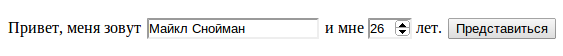
\includegraphics{08-forms-image-01.png}
\end{figure}
For these use cases, monadic forms fit the bill. They are a bit more verbose than their
applicative cousins, but this verbosity allows you to have complete control over what the
form will look like. In order to generate the form above, we could code something like
this.

\begin{lstlisting}
{-# LANGUAGE OverloadedStrings, TypeFamilies, QuasiQuotes,
             TemplateHaskell, MultiParamTypeClasses #-}

import Yesod
import Control.Applicative
import Data.Text (Text)

data MFormExample = MFormExample

mkYesod "MFormExample" [parseRoutes|
/ RootR GET
|]

instance Yesod MFormExample

instance RenderMessage MFormExample FormMessage where
    renderMessage _ _ = defaultFormMessage

data Person = Person { personName :: Text, personAge :: Int }
    deriving Show

personForm :: Html -> MForm MFormExample MFormExample (FormResult Person, Widget)
personForm extra = do
    (nameRes, nameView) <- mreq textField "this is not used" Nothing
    (ageRes, ageView) <- mreq intField "neither is this" Nothing
    let personRes = Person <$> nameRes <*> ageRes
    let widget = do
            toWidget [lucius|
##{fvId ageView} {
    width: 3em;
}
|]
            [whamlet|
#{extra}
<p>
    Hello, my name is #
    ^{fvInput nameView}
    \ and I am #
    ^{fvInput ageView}
    \ years old. #
    <input type=submit value="Introduce myself">
|]
    return (personRes, widget)

getRootR :: Handler RepHtml
getRootR = do
    ((res, widget), enctype) <- runFormGet personForm
    defaultLayout [whamlet|
<p>Result: #{show res}
<form enctype=#{enctype}>
    ^{widget}
|]

main :: IO ()
main = warpDebug 3000 MFormExample
\end{lstlisting}

Similar to the applicative areq, we use mreq for monadic forms. (And yes, there's also
mopt for optional fields.) But there's a big difference: mreq gives us back a pair of
values. Instead of hiding away the FieldView value and automatically inserting it into a
widget, we get the control to insert it as we see fit.

FieldView has a number of pieces of information. The most important is fvInput, which is
the actual form field. In this example, we also use fvId, which gives us back the HTML id
attribute of the input tag. In our example, we use that to specify the width of the field.

You might be wondering what the story is with the "this is not used" and "neither is this"
values. mreq takes a FieldSettings as its second argument. Since FieldSettings provides an
IsString instance, the strings are essentially expanded by the compiler to:

\begin{lstlisting}
fromString "this is not used" == FieldSettings
    { fsLabel = "this is not used"
    , fsTooltip = Nothing
    , fsId = Nothing
    , fsName = Nothing
    , fsClass = []
    }
\end{lstlisting}

In the case of applicative forms, the fsLabel and fsTooltip values are used when
constructing your HTML. In the case of monadic forms, Yesod does not generate any of the
"wrapper" HTML for you, and therefore these values are ignored. However, we still keep the
FieldSettings parameter to allow you to override the id and name attributes of your fields
if desired.

The other interesting bit is the extra value. GET forms include an extra field to indicate
that they have been submitted, and POST forms include a security tokens to prevent CSRF
attacks. If you don't include this extra hidden field in your form, Yesod will not accept
it.

Other than that, things are pretty straight-forward. We create our personRes value by
combining together the nameRes and ageRes values, and then return a tuple of the person
and the widget. And in the getRootR function, everything looks just like an applicative
form. In fact, you could swap out our monadic form with an applicative one and the code
would still work.

\section{Input forms}

Applicative and monadic forms handle both the generation of your HTML code and the parsing
of user input. Sometimes, you only want to do the latter, such as when there's an
already-existing form in HTML somewhere, or if you want to generate a form dynamically
using Javascript. In such a case, you'll want input forms.

These work mostly the same as applicative and monadic forms, with some differences:
\begin{itemize}
 \item You use runInputPost and runInputGet.
 \item You use ireq and iopt. These functions now only take two arguments: the field type
and the name (i.e., HTML name attribute) of the field in question.
 \item  After running a form, it returns the value. It doesn't return a widget or an
encoding type.
 \item  If there are any validation errors, the page returns an "invalid arguments" error
page.
\end{itemize}
You can use input forms to recreate the previous example. Note, however, that the input
version is less user friendly. If you make a mistake in an applicative or monadic form,
you will be brought back to the same page, with your previously entered values in the
form, and an error message explaning what you need to correct. With input forms, the user
simply gets an error message.

\begin{lstlisting}
{-# LANGUAGE OverloadedStrings, TypeFamilies, QuasiQuotes,
             TemplateHaskell, MultiParamTypeClasses #-}

import Yesod
import Control.Applicative
import Data.Text (Text)

data Input = Input

mkYesod "Input" [parseRoutes|
/ RootR GET
/input InputR GET
|]

instance Yesod Input

instance RenderMessage Input FormMessage where
    renderMessage _ _ = defaultFormMessage

data Person = Person { personName :: Text, personAge :: Int }
    deriving Show

getRootR :: Handler RepHtml
getRootR = defaultLayout [whamlet|
<form action=@{InputR}>
    <p>
        My name is #
        <input type=text name=name>
        \ and I am #
        <input type=text name=age>
        \ years old. #
        <input type=submit value="Introduce myself">
|]

getInputR :: Handler RepHtml
getInputR = do
    person <- runInputGet $ Person
                <$> ireq textField "name"
                <*> ireq intField "age"
    defaultLayout [whamlet|<p>#{show person}|]

main :: IO ()
main = warpDebug 3000 Input
\end{lstlisting}

\section{Custom fields}

The fields that come built-in with Yesod will likely cover the vast majority of your form
needs. But occassionally, you'll need something more specialized. Fortunately, you can
create new forms in Yesod yourself. The Field datatype has two records: fieldParse takes a
list of values submitted by the user and returns one of three results:
\begin{enumerate}
 \item An error message saying validation failed.
 \item The parsed value.
 \item Nothing, indicating that no data was supplied.
\end{enumerate}

That last case might sound surprising: shouldn't Yesod automatically know that no
information is supplied when the input list is empty? Well, no actually. Checkboxes, for
instance, indicate an unchecked state by sending in an empty list.

Also, what's up with the list? Shouldn't it be a Maybe? Well, that's also not the case.
With grouped checkboxes and multi-select lists, you'll have multiple widgets with the same
name. We also use this trick in our example below.

The second record is fieldView, and it renders a widget to display to the user. This
function has four arguments: the id attribute, the name attribute, the result and a Bool
indicating if the field is required.

What did I mean by result? It's actually an Either, giving either the unparsed input (when
parsing failed) or the successfully parsed value. intField is a great example of how this
works. If you type in 42, the value of result will be Right 42. But if you type in turtle,
the result will be Left "turtle". This lets you put in a value attribute on your input tag
that will give the user a consistent experience.

As a small example, we'll create a new field type that is a password confirm field. This
field has two text inputs- both with the same name attribute- and returns an error message
if the values don't match. Note that, unlike most fields, it does not provide a value
attribute on the input tags, as you don't want to send back a user-entered password in
your HTML ever.

\begin{lstlisting}
passwordConfirmField :: Field sub master Text
passwordConfirmField = Field
    { fieldParse = \rawVals ->
        case rawVals of
            [a, b]
                | a == b -> return $ Right $ Just a
                | otherwise -> return $ Left "Passwords don't match"
            [] -> return $ Right Nothing
            _ -> return $ Left "You must enter two values"
    , fieldView = \idAttr nameAttr _ eResult isReq -> [whamlet|
<input id=#{idAttr} name=#{nameAttr} type=password>
<div>Confirm:
<input id=#{idAttr}-confirm name=#{nameAttr} type=password>
|]
    }

getRootR :: Handler RepHtml
getRootR = do
    ((res, widget), enctype) <- runFormGet $ renderDivs
        $ areq passwordConfirmField "Password" Nothing
    defaultLayout [whamlet|
<p>Result: #{show res}
<form enctype=#{enctype}>
    ^{widget}
    <input type=submit value="Change password">
|]
main :: IO ()
main = warpDebug 3000 Password
\end{lstlisting}

\section{Заключение}

Формы в Yesod делятся на три вида. Аппликативные используются чаще всего, так как
предоставляют красивый интерфейс и простой для использование API. Монадические форма дают
больше возможностей, но их сложнее использовать. Формы ввода данных полезны, когда вам
надо просто принять данные пользователя, не генерируя сложных виджетов.

Из коробки Yesod предоставляет несколько видов полей для форм. Для использования
форм вам придется определиться, какую форму вы хотите и является поле опциональным или
обязательным. Итого мы имеет шесть дополнительных функций: areq, aopt, mreq, mopt, ireq,
и iopt.

Формы довольно-таки мощны. Они могут автоматически вставлять код на Javascript, чтобы
получаять более красивые элементы управляения, например, для выбора даты из библиотеки 
jQuery. Формы также поддерживают  i18n, так что вы можете расчитывать на большое
сообщество пользователей. А для более специфических надобностей, вы можете привязать
функции валидации данных для конкретных полей, или написать свои с чистого  листа.

